\chapter{Krigagem}

\section{Introdução} \label{secao1}

A krigagem é um termo genérico que expressa um conjunto de metodologias de estimativa que levam em consideração o mínimo valor do erro. Os métodos também são chamados de BLUE ( Best linear umbiesed estimation). Entre os procedimentos podemos citar a krigagem ordinária, krigagem simples, krigagem da probabilidade e krigagem universal. Algumas metodologias não lineares tais como a krigagem de indicadores e a krigagem gaussiana também recebem o mesmo nome, pois utilizam operações lineares em dados transformados. 

É importante entender, antes de tudo, que estimar é um processo sempre associado ao erro. O que é possível de se fazer durante uma estimativa é sempre reduzí-lo ao máximo e encontrar o valor mais provável de ocorrência. No entanto, se um evento tem baixa probabilidade, como ganhar em uma sena, ainda sim há pessoas que por hora ganham no jogo. Da mesma forma se algo possui grande probabilidade de ocorrer, como um lutador de boxe ganhar em uma luta contra um menino de cinco anos, ainda sim podemos nos surpreender.

Na krigagem utilizamos um estimador para determinar a realização de uma variável aleatória em um ponto desconhecido. Este é uma combinação linear de vários valores de amostras ao redor do ponto a ser estimado \eqref{krig_estm}

\begin{equation}\label{krig_estm}
z_{0} = \sum_{i=1}^{n} \lambda_{i} z_{i} 
\end{equation}

Em que $\lambda_{i}$ são valores de peso associados a cada uma das amostras utilizadas para a estimativa. Não utilizamos todas as amostras do domínio, porque primeiramente, causará uma grande suavização nas estimativas e em segundo, porque computacionalmente é melhor realizar o filtro nos dados e inverter matrizes de krigagem pequenas, do que inverter matrizes de krigagem grandes. O tempo de krigagem de subproblemas não é diretamente proporcional a de grandes problemas. 


Como demonstrado no capíulo um podemos definir o erro de estimativa segundo a equação \eqref{krig1}

\begin{equation}\label{krig1}
\varepsilon (z^{*}_{0}) = z^{*}_{0} -z_{0} 
\end{equation}

Em que $z^{*}_{0}$ é o valor estimado no ponto desconhecido e $z_{0}$ é o valor real naquele ponto. Substituindo a equação \eqref{krig_estm} em \eqref{krig1} obtemos a relação \eqref{krig2}

\begin{equation}\label{krig2}
\varepsilon (z^{*}_{0}) = \sum_{i=1}^{n} \lambda_{i} z_{i}  -z_{0} 
\end{equation}

Tomando o quadrado do erro de estimativa temos a seguinte a relação \eqref{krig3}

\begin{equation}\label{krig3}
\varepsilon (z^{*}_{0})^2 = \sum_{i=1}^{n} \lambda_{i} \sum_{i=j}^{n} \lambda_{j}z_{i}z_{j} -2\sum_{i=1}^{n} \lambda_{i}z_{i}z_{0} -z_{0}^2 
\end{equation}

Tomando o menor valor esperado do erro quadrádico temos então 

\begin{equation}\label{krig4}
E\left(\varepsilon (z^{*}_{0})^2\right) = \sum_{i=1}^{n} \lambda_{i} \sum_{j=1}^{n} \lambda_{j}Cov(z_{i},z_{j}) -2\sum_{i=1}^{n} \lambda_{i}Cov(z_{i},z_{0}) -Cov(z_{0},z_{0}) 
\end{equation}

Que também é chamada variância de extensão. Ou seja, esta é uma estimativa de quanto varia tomarmos como valor de um ponto desconhecido uma combinação linear de valores mais próximos dele. Para encontrarmos a variância de krigagem precisamos minimizar esta variância de extensão, adicionando a condição de não viés da estatística. Como demonstrado no capítulo \ref{Cap_4} no subitem \ref{demons_krig} a condição de não viés amostral neste caso é que a soma dos ponderadores deve ser igual a 1.

Adicionando a restrição no problema e tomando as derivadas parciais para cada um das equações consideradas temos a relação demonstrada por \eqref{krig4} 

\begin{equation}\label{krig5}
\sigma ^2_{krig} = \frac{\partial }{\partial \lambda _{i}} \left( \sum_{i=1}^{n} \lambda_{i} \sum_{j=1}^{n} \lambda_{j}Cov(z_{i},z_{j}) -2\sum_{i=1}^{n} \lambda_{i}Cov(z_{i},z_{0}) -Cov(z_{0},z_{0}) \right ) + \frac{\partial }{\partial \lambda _{i}} R = 0 | \forall i
\end{equation}

Em que R é a restrição de não enviesamento adicionado ao problema, associada a soma dos ponderadores da krigagem. Tomando o valor das derivadas parciais temos o seguinte conjunto de equações \eqref{krig6}

 \begin{equation}\label{krig6}
 \sigma ^2_{krig} =  2\sum_{i=1}^{n} \lambda_{i}  Cov(z_{i},z_{j}) -2Cov(z_{i},z_{0})  + \frac{\partial }{\partial \lambda _{i}} R = 0 | \forall i
 \end{equation}

O cálculo das derivadas parciais pode ser realizado de acordo com a expansão dos somatórios como demonstrado na equação \eqref{krig4}

\begin{equation}\label{krig7}
 \sum_{i=1}^{n}  \sum_{j=1}^{n} \lambda_{j} \lambda_{i} Cov(z_{i},z_{j}) =   \sum_{j=2}^{n} \lambda_{j} \lambda_{1} Cov(z_{1},z_{j})  + \sum_{i=2}^{n} \lambda_{1} \lambda_{i}  Cov(z_{i},z_{1})  + \lambda_{1}\lambda_{1} Cov(z_{1},z_{1})
\end{equation}

Cada sistema de krigagem pode então ser resolvido de acordo com uma matriz de covariâncias genérica como descrito em \eqref{krig5}

\begin{equation}\label{krig8}
\begin{pmatrix}
Cov(z_{1},z_{1})&Cov(z_{1},z_{2})& ... & Cov(z_{1},z_{n})& \frac{\partial R }{\partial \lambda _{1}}\\ 
Cov(z_{2},z_{1})&Cov(z_{2},z_{2})& ... & Cov(z_{2},z_{n})& \frac{\partial R }{\partial \lambda _{2}}\\ 
...&...& ...&... & ...\\
Cov(z_{n},z_{1})&Cov(z_{n},z_{2})& ... & Cov(z_{n},z_{n})& \frac{\partial R }{\partial \lambda _{n}}\\
1&1& 1&...& 0
\end{pmatrix} 
\begin{pmatrix}
\lambda _{1}\\ 
\lambda _{2}\\ 
...\\ 
\lambda _{n}\\
1/2
\end{pmatrix}=\begin{pmatrix}
Cov(z_{0}, z{1})\\ 
Cov(z_{0}, z{2})\\  
...\\
Cov(z_{0}, z{n})\\
P
\end{pmatrix}
\end{equation}

Em que P é o valor da restrição para a soma dos ponderadores. O termo da esquerda da matriz é responsável pelo desagrupamento dos dados, enquanto o termo da direita é responsável por ponderar a distância do ponto estimado até a amostra considerada. Esse sistema de matrizes proposto aqui é genérico, e qualquer krigagem pode ser descrita a partir dele, bastando apenas considerar diferentes variáveis e funções de restrição ao enviesamento R e o valor P de restrição à soma dos ponderadores. Nos tópicos a seguir demonstraremos as restrições quanto a krigagem ordinária e simples. Encontrados os pesos da krigagem podemos encontrar o valor estimado pela equação \eqref{krig1}

\section{Krigagem Ordinária}

 Para a krigagem ordinária utilizamos os mesmos pressupostos e cálculos utilizados em \ref{secao1}. Logo temos como restrição à condição de não viés dado pela demonstração abaixo:
 
 \begin{proof}
    	$Z_{0} = \sum_{i=1}^{n} \lambda_{i} Z_{i} $\\
    	$E(Z_{0}) = E\left(\sum_{i=1}^{n} \lambda_{i} Z_{i}\right) =m $\\
    	$E(Z_{0}) =\sum_{i=1}^{n}  E\left(\lambda_{i} Z_{i}\right) = m $\\
    	$E(Z_{0}) =\sum_{i=1}^{n}  \lambda_{i} E\left(Z_{i}\right) = m $\\
    	$E(Z_{0}) =\sum_{i=1}^{n}  \lambda_{i} m = m $\\
    	$m\sum_{i=1}^{n}  \lambda_{i} = m $\\
    	$\sum_{i=1}^{n}  \lambda_{i} = 1 $\\
 \end{proof}
 
 Logo nossa função de restrição pode ser determinada por \eqref{krig9}, e o nosso valor P é igual a 1.
 
 \begin{equation}\label{krig9}
 R_{i} = \mu \left( \sum_{i=0}^{n} \lambda_{i} - 1\right) | \forall i
 \end{equation} 

 Em que $\mu$ é o multipliador langragiano. Logo tomando a derivada parcial de cada uma das restrições para cada uma das amostras i do problema temos a relação segundo a equação \eqref{krig10}
 
 \begin{equation}\label{krig10}
 \frac{\partial}{\partial \lambda_{i}}R_{i} = \mu | \forall i 
 \end{equation} 
 
 O sistema de equações da krigagem pode ser transformado então na relação \ref{krig11}
 
  \begin{equation}\label{krig11}
  \begin{pmatrix}
  Cov(Z_{1},Z_{1})&Cov(Z_{1},Z_{2})& ... & Cov(Z_{1},Z_{n})& 1\\ 
  Cov(Z_{2},Z_{1})&Cov(Z_{2},Z_{2})& ... & Cov(Z_{2},Z_{n})& 1 \\ 
  ...&...& ...&... & ...\\
  Cov(Z_{n},Z_{1})&Cov(Z_{n},Z_{2})& ... & Cov(Z_{n},Z_{n})& 1\\
  1&1& 1&1& 0
  \end{pmatrix} 
  \begin{pmatrix}
  \lambda _{1}\\ 
  \lambda _{2}\\ 
  ...\\ 
  \lambda _{n}\\
  1/2\mu
  \end{pmatrix}=\begin{pmatrix}
  Cov(Z_{0}, Z_{1})\\ 
  Cov(Z_{0}, Z_{2})\\  
  ...\\
  Cov(Z_{0}, Z_{n})\\
  1
  \end{pmatrix}
  \end{equation}

\section{Krigagem Simples}

A krigagem simples tem como pressuposto encontrar os ponderadores que minimizem o resíduo da variável aleatória. Como determinado em \ref{residuo}, nada mais é que a própria variável subtraído do valor médio da função aleatória. Logo o método requer antes de tudo conhecimento do valor médio  e da hipótese de estacionaridade de segunda ordem. Neste caso temos que o valor estimado pode ser descrito pela equação \eqref{krig12}  

 \begin{equation}\label{krig12}
 Z^*_{0} = \sum_{i=0}^{n} \lambda_{i}\left( Z_{i} - m \right) + m
 \end{equation}
 
 Podemos isolar os termos da equação \eqref{krig6} em relação ao valor médio assim obtendo a equação \eqref{krig13}
 
 \begin{equation}\label{krig13}
 Z^*_{0} = \sum_{i=0}^{n} \lambda_{i} Z_{i} + m\left(1- \sum_{i=0}^{n}\lambda_{i} \right)
 \end{equation} 

Ou seja, notamos que na krigagem simples parte dos pesos é atribuído à variável aleatória e parte para a média global. Considerando a condição de não viés amostral temos que a soma dos ponderadores deve ser igual a zero 

\begin{proof}
$E\left(Z^*_{0}\right) = E\left(\sum_{i=0}^{n} \lambda_{i}Y_{0} + m \right) = m $\\
$E\left(Z^*_{0}\right) = \sum_{i=0}^{n} \lambda_{i}E\left( Y_{0} \right) + E(m) = m $\\
$\sum_{i=0}^{n} \lambda_{i}E\left( Y_{0} \right) + m = m $\\
$\sum_{i=0}^{n} \lambda_{i}E\left( Y_{0} \right)  = 0 $\\
$E\left( Y_{0} \right)  = 0 \vee \sum_{i=0}^{n} \lambda_{i} = 0 $
\end{proof}

Caso a escolha da média da função aleatória seja realmente correta e o caso perfeitamente estacionário nenhuma condição seria necessária para o não enviesamento da estatística. No entanto, para forçarmos o sistema de resolução das matrizes de krigagem encontrar valores condizentes optamos por adicionar a condição de que a soma dos ponderadores deve ser igual a zero. Em outras palavras, diferentemente da krigagem ordinária, a krigagem simples pressupõe o conhecimento intrínseco da média da função aleatória, o que na maioria das vezes não é realidade.

Nossa função de restrição se torna portanto a equação \eqref{krig14} e o nosso valor P de restrição à soma dos ponderadores é igual a 0.

\begin{equation}\label{krig14}
R_{i} = \mu \sum_{i=0}^{n} \lambda_{i} | \forall i
\end{equation}   

Em que $\mu$ é o multiplicador lagrangiano. Tomando a derivada parcial de cada restrição para cada índice temos que

\begin{equation}\label{krig15}
\frac{\partial}{\partial \lambda_{i}}R_{i} = \mu | \forall i 
\end{equation} 


Logo o sistema de matrizes para  a krigagem simples pode ser transformado em \eqref{krig16}

\begin{equation}\label{krig16}
\begin{pmatrix}
Cov(Y_{1},Y_{1})&Cov(Y_{1},Y_{2})& ... & Cov(Y_{1},Y_{n})& 1\\ 
Cov(Y_{2},Y_{1})&Cov(Y_{2},Y_{2})& ... & Cov(Y_{2},Y_{n})& 1 \\ 
...&...& ...&... & ...\\
Cov(Y_{n},Y_{1})&Cov(Y_{n},Y_{2})& ... & Cov(Y_{n},Y_{n})& 1\\
1&1& 1&1& 0
\end{pmatrix} 
\begin{pmatrix}
\lambda _{1}\\ 
\lambda _{2}\\ 
...\\ 
\lambda _{n}\\
1/2\mu
\end{pmatrix}=\begin{pmatrix}
Cov(Y_{0}, Y_{1})\\ 
Cov(Y_{0}, Y_{2})\\  
...\\
Cov(Y_{0}, Y_{n})\\
0
\end{pmatrix}
\end{equation}

Sendo a covariância dos resíduos a mesma covariância das amostras. Calculado os pesos de cada um dos resíduos encontramos o valor estimado.

\section{Krigagem de blocos}

Um caso especial de krigagem ocorre quando o variável estimada tem um suporte diferente das amostras. A forma mais simples de se resolver este problema é estimando uma série de valores dentro do suporte a ser estimado e tomando seu valor médio. A figura \eqref{krig13f} demonstra um bloco B contendo novo pontos k1 até k9 contidos nele. 

\begin{figure}[H]
	\centering
	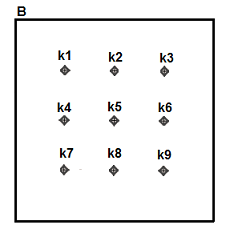
\includegraphics[scale=1.0]{krig13.png}
	\caption{Demonstração dos pesos de krigagem para o posicionamento de amostras para um modelo de pepita puro}
	\label{krig13f}
\end{figure}

Neste caso o valor da variável aleatória para o suporte estimado pode ser dado por uma média das combinações lineares de variáveis pontuais contidas dentro da região a ser estimada tal como em \eqref{krig17}

\begin{equation}\label{krig17}
Z_{v}  = \frac{1}{p}\sum_{j=1}^{p} Z_{j}
\end{equation}

Em que p é o número de variáveis contidas dentro daquele volume. Logo temos o erro de estimativa dado pela equação \eqref{krig18}

\begin{equation}\label{krig18}
\varepsilon (Z^{*}_{v}) = Z^{*} _{v} - Z_{v}
\end{equation}

\begin{proof}
	$\varepsilon (Z^{*}_{v}) = \frac{1}{p}\sum_{j=1}^{p}(\sum_{i=1}^{n}\lambda_{i}Z_{i} -  Z_{j}) $ \\
	$\varepsilon (Z^{*}_{v}) = \frac{1}{p}\sum_{j=1}^{p}\sum_{i=1}^{n}\lambda_{i}Z_{i} - \frac{1}{p}\sum_{j=1}^{p} Z_{j} $ \\
	$\varepsilon (Z^{*}_{v}) = \frac{1}{p}p\sum_{i=1}^{n}\lambda_{i}Z_{i} - \frac{1}{p}\sum_{j=1}^{p} Z_{j} $\\	
	$\varepsilon (Z^{*}_{v}) = \sum_{i=1}^{n}\lambda_{i}Z_{i} - \frac{1}{p}\sum_{j=1}^{p} Z_{j} $\\	
	$\varepsilon (Z^{*}_{v})^2 = \sum_{i=1}^{n}\sum_{i'=1}^{n}\lambda_{i}\lambda_{i'}Z_{i}Z_{i'} - \frac{2}{p}\sum_{i=1}^{n}\sum_{j=1}^{p}\lambda_{i}Z_{i}Z_{j}+ \frac{1}{p^2}\sum_{j=1}^{p}\sum_{j'=1}^{p} Z_{j}Z_{j'} $\\
	$E\left(\varepsilon (Z^{*}_{v})^2 \right) = \sum_{i=1}^{n}\sum_{i'=1}^{n}\lambda_{i}\lambda_{i'}Cov(Z_{i},Z_{i'}) - \frac{2}{p}\sum_{i=1}^{n}\sum_{j=1}^{p}\lambda_{i}Cov(Z_{i}Z_{j})+ \frac{1}{p^2}\sum_{j=1}^{p}\sum_{j'=1}^{p} Cov(Z_{j}Z_{j'}) $\\   
     Derivando em relação ao ponderador tal como demonstrado na seção anterior encontramos a seguinte equação para a variância de krigagem:    \\
     $\sigma^{2}_{krig} = 2\sum_{i'=1}^{n}\lambda_{i'}Cov(Z_{i},Z_{i'}) - \frac{2}{p}\sum_{j=1}^{p}Cov(Z_{i}Z_{j}) |\forall i $\\   
     Em que: \\    
     $\overline{Cov}(Z_{i}Z_{j}) = \frac{1}{p}\sum_{j=1}^{p}Cov(Z_{i}Z_{j})$\\
     Logo temos: \\
	 $\sigma^{2}_{krig} = 2\sum_{i=1'}^{n}\lambda_{i}Cov(Z_{i},Z_{i'}) - 2\overline{Cov}(Z_{i}Z_{j}) |\forall i $\\ 
	 
	 
\end{proof}

Ou seja, se estamos estimando um bloco a partir de um ponto, a única diferença entre o sistema de krigagem convencional é que o lado da direita da matriz é substituído pela média das covariâncias entre cada amostra e os pontos estimados dentro do bloco. A figura \eqref{krig14f} demonstra como deve-se proceder para calcular a covariância média para cada amostra na krigagem de blocos.

\begin{figure}[H]
	\centering
	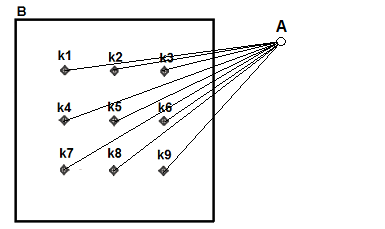
\includegraphics[scale=1.0]{krig14.png}
	\caption{Covariância média como a média de covariâncias entre cada ponto estimado k dentro do bloco e o valor de cada amostra A}
	\label{krig14f}
\end{figure}

Logo o sistema de krigagem para blocos é demonstrado em \eqref{krig19}

  \begin{equation}\label{krig19}
  \begin{pmatrix}
  Cov(Z_{1},Z_{1})&Cov(Z_{1},Z_{2})& ... & Cov(Z_{1},Z_{n})& 1\\ 
  Cov(Z_{2},Z_{1})&Cov(Z_{2},Z_{2})& ... & Cov(Z_{2},Z_{n})& 1 \\ 
  ...&...& ...&... & ...\\
  Cov(Z_{n},Z_{1})&Cov(Z_{n},Z_{2})& ... & Cov(Z_{n},Z_{n})& 1\\
  1&1& 1&1& 0
  \end{pmatrix} 
  \begin{pmatrix}
  \lambda _{1}\\ 
  \lambda _{2}\\ 
  ...\\ 
  \lambda _{n}\\
  1/2\mu
  \end{pmatrix}=\begin{pmatrix}
  \overline{Cov}(Z_{0}, Z_{1})\\ 
  \overline{Cov}(Z_{0}, Z_{2})\\  
  ...\\
  \overline{Cov}(Z_{0}, Z_{n})\\
  1
  \end{pmatrix}
  \end{equation}

\section{Influência nos pesos da krigagem}

A krigagem é na verdade um estimador que não leva em consideração o valor da ammostra, mas apenas sua correlação espacial e disposição no espaço das amotras. Essa é a grande crítica aos métodos de krigagem que atualmente estão sendo substituídos aos poucos pelos métodos de simulação geoestatística. Mostraremos a influência nos pesos da krigagem quanto a disposição espacial quanto ao modelo de continuidade espacial adotado e quanto ao posicionamento das amostras. 

\subsection{Influência do modelo de continuidade espacial nos pesos}

A figura \eqref{krig1f} demonstra o posicionamento de quatro amostras em relação ao ponto estimado. As amostras no sentido vertical da figura estão mais próximas que no sentido horizontal. Quando considerado um modelo de pepita puro, os pesos de krigagem são sempre os mesmos independente do posicionamento das amostras.

\begin{figure}[H]
  	\centering
  	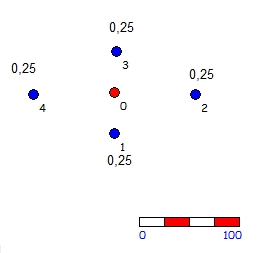
\includegraphics[scale=1.0]{krig1.png}
  	\caption{Demonstração dos pesos de krigagem para o posicionamento de amostras para um modelo de pepita puro}
  	\label{krig1f}
\end{figure}

A figura \eqref{krig2f} demonstra o mesmo caso para um modelo esférico. O range adotado é igual a 2L. O modelo esférico e exponencial tende a dar pesos diferenciados para as amostras mais próximas, tal que seu valor é maior quanto mais próxima for a amostra do ponto a ser estimado. 

\begin{figure}[!]
  	\centering
  	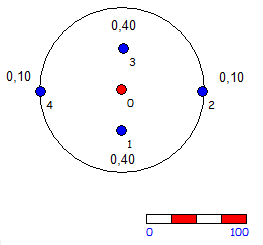
\includegraphics[scale=1.0]{krig2.png}
  	\caption{Demonstração dos pesos de krigagem para o posicionamento de amostras em um modelo esférico com alcance igual a 2L. A linha cheia representa o alcance do variograma}
  	\label{krig2f}
\end{figure}

A figura \eqref{krig3f} demonstra o mesmo caso para um modelo gaussiano. O range prático adotado é de 1.5 L. O modelo gaussiano é sem dúvida o mais suavizador de todos os outros modelos para a krigagem, considerando seu comportamento parabólico  próximo à origem. Maiores pesos são atribuídos às distâncias mais proximais. 


\begin{figure}[!]
  	\centering
  	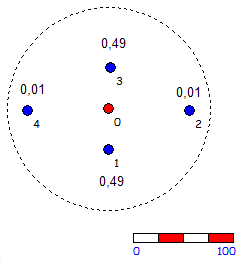
\includegraphics[scale=1.0]{krig3.png}
  	\caption{Demonstração dos pesos de krigagem para o posicionamento de amostras em um modelo gaussiano com alcance igual a 1.5L. A linha hachurada demonstra o alcance prático do modelo de continuidade espacial.}
  	\label{krig3f}
\end{figure}

\subsection{Influência dos parâmetros do variograma}

O alcance do variograma altera os pesos de krigagem aumentando os valores das amostras mais próximas para um aumento do mesmo. A figura \eqref{krig4f} demonstra os pesos de krigagem para um modelo esférico de variograma com um alcance de 63m e outro de 125m. As amostras estão dispostas em uma cruz com o ponto estimado tal que o eixo maior possui 162m e o eixo menor igual a 80m. 

\begin{figure}[H]
   	\centering
   	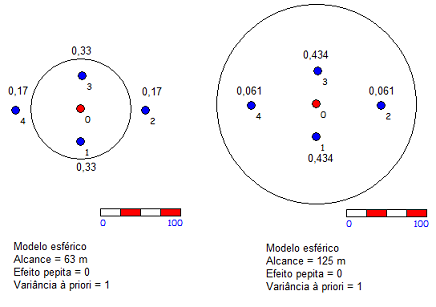
\includegraphics[scale=0.8]{krig4.png}
   	\caption{Influência dos parâmetros do variograma na krigagem. Efeito do alcance. Maiores alcances atribuem mais peso à amostras mais próximas}
   	\label{krig4f}
\end{figure}

Quanto a variância à priori do variograma notamos segundo a figura \eqref{krig5f} que qualquer valor adicionado não altera os pesos de krigagem. No entanto, apesar de não alterar os pesos, um aumento na variância à priori causa um aumento na variância de krigagem. 

\begin{figure}[H]
  	\centering
  	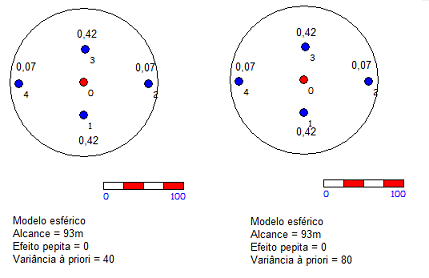
\includegraphics[scale=0.8]{krig5.png}
  	\caption{Influência dos parâmetros do variograma na krigagem. Efeito da variância a priori. Maiores valores de variância não alteram os pesos das amostras}
  	\label{krig5f}
\end{figure}

Em último caso notamos segundo a figura \eqref{krig6f} que o efeito pepita tende a normalizar os pesos de krigagem. Quanto maior for o efeito pepita e menor a contribuição, mais o modelo de variograma se aproxima de efeito pepita puro e neste caso qualquer geometria das amostras produzirá pesos iguais. 

\begin{figure}[H]
	\centering
	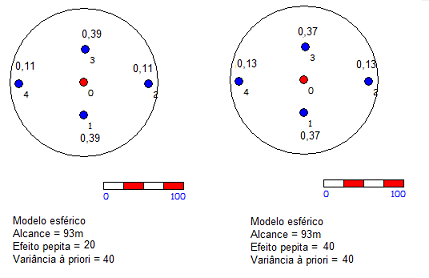
\includegraphics[scale=0.8]{krig6.png}
	\caption{Influência dos parâmetros do variograma na krigagem. Efeito do alcance. Maiores alcances atribuem mais peso à amostras mais próximas}
	\label{krig6f}
\end{figure}

\subsection{Efeito da geometria das amostras}

Quanto a geometria das amostras é necessário lembrar que distâncias iguais entre as amostras e o ponto estimado produzem pesos iguais, no caso de um modelo de continuidade espacial isotrópico. A figura \eqref{krig7f} demonstra esta relação.

\begin{figure}[H]
	\centering
	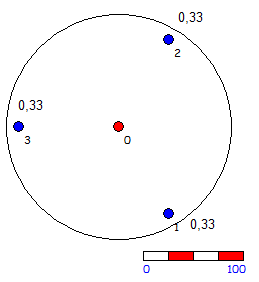
\includegraphics[scale=0.8]{krig7.png}
	\caption{Influência no peso para distâncias iguais das amostras ao ponto estimado. Pesos iguais para um modelo de continuidade espacial isotrópico.}
	\label{krig7f}
\end{figure}

Para amostras agrupadas a tendência é produzir pesos iguais. A figura \eqref{krig8f} demonstra esta situação.

\begin{figure}[H]
	\centering
	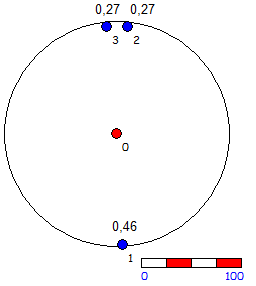
\includegraphics[scale=0.8]{krig8.png}
	\caption{Influência de amostras agrupadas nos pesos da krigagem. Tendência de valores iguais para os pesos. }
	\label{krig8f}
\end{figure}

O caso mais importante para o posicionamento das amostras é quando existem amostras à frente de outras. Nesse caso ocorre "blindagem" e é possível que elas recebam pesos negativos. O termo em inglês para isto é "screen effect". Pesos negativos para um valor estimado são comuns de ocorrer, o que não é adequado muitas vezes é um valor negativo para estimativas, quando a variável somente pode assumir valores positivos. Neste caso é importante um controle sobre a estratégia de busca de forma a garantir a melhor situação para ponderadores negativos. A figura \eqref{krig9f} demonstra o feito de blindagem das amostras e associação com pesos negativos. 

\begin{figure}[H]
	\centering
	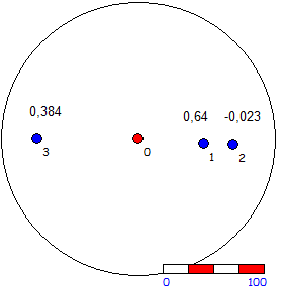
\includegraphics[scale=0.8]{krig9.png}
	\caption{Influência da blindagem de amostras. Pesos negativos para amostras que estão encobertas por outras. }
	\label{krig9f}
\end{figure}
 
Outra variável importante que influencia no peso da krigagem é o suporte do valor estimado. Neste caso estamos lidando com um tipo diferente de krigagem também chamada de krigagem de blocos ao qual o suporte estimado é diferente do suporte das amostras. Blocos maiores tendem neste caso a normalizar o peso das amostras, mas nunca a igualá-los tal como acontece com o modelo de efeito pepita puro. A figura \eqref{krig10f} tende a demonstrar esta situação. 

\begin{figure}[H]
	\centering
	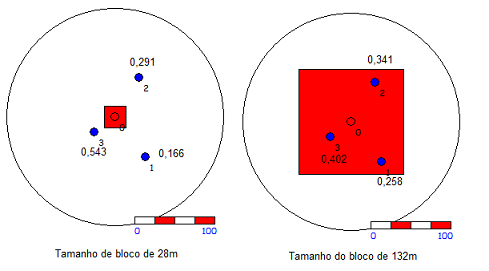
\includegraphics[scale=0.8]{krig10.png}
	\caption{Influência do efeito de suporte do valor estimado. Blocos maiores tendem a normalizar o peso das amostras.  }
	\label{krig10f}
\end{figure}


\section{Estratégia de procura}

Como dito anteriormente a krigagem exige que determinemos uma região envolta do ponto a ser estimado que determinará as amostras que ponderarão a estimativa. Escolher uma região muito pequena poderá fazer com que o algoritmo não encontre nenhuma amostra. Escolher uma região muito maior poderá suavizar a estimativa a ponto de tornar o valor da amostra muito próximo da média global. A escolha da estratégia de busca ideal é um fator muito mais influente muitas vezes do que um ajuste mais apurado no modelo de continuidade espacial. 

Diversas geometrias podem ser escolhidas para se realizar a estratégia de procura dos pontos, mas as mais importantes são sem dúvida a circular e a elíptica. Buscas em caixa também podem ser feitas. 

Dentre os parâmetros de krigagem mais utilizados são: 

\begin{itemize}
  	\item Número máximo e número mínimo de amostras dentro da região de busca
  	\item Forma, dimensão e orientação da região de busca
  	\item Uso de estratégia de busca por octantes
\end{itemize} 

Na maioria dos algoritmos de krigagem, a escolha definido a região de busca, caso o ponto a ser estimado esteja envolta de um número menor que o mínimo de amostras ou máximo aquele ponto simplesmente não é estimado.

Quanto a forma, dimensão e orientação da região de busca é importante lembrar que dimensões muito grandes produzirão grande suavização nos valores krigados, o que pode não corresponder com a realidade. Valores muito pequenos, no entanto, podem atribuir poucos pontos na estimativa e torná-la também inadequada. 

Uma das formas utilizadas para reduzir a suavização da krigagem é utilizar uma estratégia de busca elíptica perpendicular à continuidade espacial dos dados. Dessa forma temos duas forças contrárias agindo para garantir maior homogeneidade aos pesos e maior erraticidade aos valores estimados. A figura \eqref{krig11f} demonstra esta situação.  

\begin{figure}[H]
	\centering
	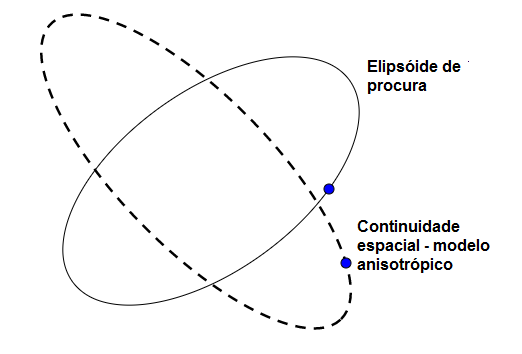
\includegraphics[scale=0.8]{krig11.png}
	\caption{Estratégia de busca perpendicular à continuidade do fenômeno. Forma utilizada para garantir maior erraticidade aos dados estimados.  }
	\label{krig11f}
\end{figure}

Outra forma de se realizar a estratégia de busca para a krigagem é utilizando octantes. Dessa forma podemos estipular um número mínimo ou máximo de amostras por cada octante para ser utilizado durante a krigagem. Uma conduta coerente é ser condizente com o número mínimo e máximo de amostras utilizada para a krigagem em cada octante. Se em uma estimativa usa-se um número mínimo de 8 amostras para a krigagem e 32 como o máximo, é plausível escolher uma estratégia de octantes que utilize um mínimo de 1 amostra por octante e no máximo 4. A figura \eqref{krig12f} demonstra a estratégia de octantes para o caso considerado. Se o número mínimo de amostras por octante fosse de 3 amostras, os octantes 1,4,6 e 7 estariam descartados. 

\begin{figure}[H]
	\centering
	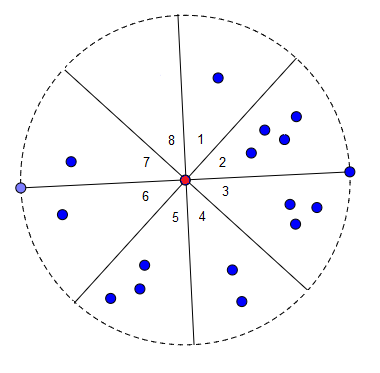
\includegraphics[scale=0.8]{krig12.png}
	\caption{Estratégia de busca por octantes. Octantes 1,4,6 e 7 descartados por não possuírem o mínimo de amostras igual a 3 }
	\label{krig12f}
\end{figure}

\section{Validação da krigagem}

Após realizada a krigagem devemos investigar se os valores estimados estão realmente próximos do esperado. Algumas metodologias são utilizadas para isso, entre elas citamos:

\begin{enumerate} 
	\item Verificação do comportamento dos mapas krigado e das amostras
	\item Comparação da média global com a média das amostras
	\item Análise de deriva de bandas do mapa 
	\item Validação Cruzada
	\item Verificação de pesos negativos	
\end{enumerate}

\subsection{Verificação do comportamento dos mapas krigado e das amostras}

É importante que o mapa de valores krigados apresente comportamento semelhante das amostras. Nesta etapa verifica-se se a continuidade dos dados estimados é visualmente condizente com as características do fenônmeno estudado, tal como continuidade espacial e regiões de maior ou menor valor da variável aleatória. 

A figura \eqref{krig15f} demonstra a comparação visual entre um mapa realizado por polígonos de influência da amostra e outro krigado. Nota-se que em ambos a continuidade espacial dos dados apresenta direção NW e que as regiões de maior e menor valor são semelhantes.

\begin{figure}[H]
	\centering
	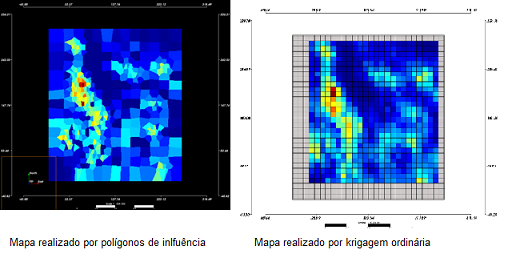
\includegraphics[scale=0.8]{krig15.png}
	\caption{Comparação visual entre os valores da amostra por polígono de influência e dos blocos krigados.}
	\label{krig15f}
\end{figure}

\subsection{Comparação da média global com a média das amotras}

A krigagem é uma estatística não enviesada, isso significa que a média das amostras deve ser idêntica à media dos valores krigados. No entanto, a variância dos valores krigados é menor que a variância das amostras devido o efeito de suporte. 

\subsection{Análise de deriva de bandas do mapa}

Não obstante a média das amostras deve ser a média do valor krigado, a média em subdomínios do mapa krigado deve ser igual a média dos subdomínios das amostras. Para isso realizamos um gráfico como demonstrado na figura \eqref{krig16f}. Dividimos o domínio espacial das amostras e dos valores krigado em bandas e tomamos os valores médios de cada banda colocando em um gráfico. Se o comportamento das duas curvas for semelhante falhamos em aceitar a hipótese de deriva nos dados. As bandas no gráfico podem ser analisadas nas diferentes direção de independência dos eixos cartesianos.


\begin{figure}[H]
	\centering
	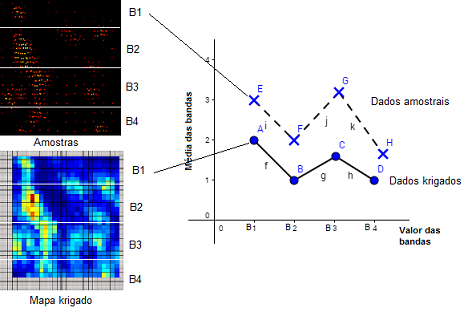
\includegraphics[scale=0.8]{krig16.png}
	\caption{Exemplo da análise de deriva. Mama dos valores krigados e das amostras dividido em bandas e média tomaada para cadab banda em cada mapa demonstrado ao lado. Comportamento do gráfico semelhantne para as duas situações. Descarte da hipótese de deriva.}
	\label{krig16f}
\end{figure}

\subsection{Validação cruzada}

A validação cruzada é uma estimativa do erro de krigagem possível. Para isso retiramos um ponto amostral e estimamos sem aquele dado no ponto novamente. A diferença entre o valor estimado e o valor real da amostra é uma medida de erro, com média zero e variância determinada pelo conjunto de amostras. A validação cruzada não é necessariamente um valor de erro real cometido pelo método, mas uma alternativa comparativa entre diferentes modelos de continuidade espacial e estratégia de busca. Antes de realizar a krigagem, é interessante testar valores de validação cruzadas diferentes para encontrar a melhor estratégia de busca. 

\subsection{Verificação de pesos negativos}

Como dito nas seções anteriores amostras blindadas podem produzir pesos negativos na krigagem. É interessante controlar a quantidade de pesos negativo na estimativa a fim de produzir um resultado com menor suavização. Para reduzir a quantidade de pesos negativos opta-se por reduzir o tamanho da região de busca de amostras na krigagem. 

\begin{exercise}
	A figura abaixo demonstra 3 pontos amostras e um ponto a ser estimado z0. Considere o modelo de continuidade espacial como: \\
	
	\vspace{0.5cm}
	 $\\gamma (h) = \begin{pmatrix}
	12\left(\left [ \frac{3h}{4} \right ]-\left [ \frac{h^{3}}{64} \right ]\right), h\leqslant 4\\
	12,h> 4
	
	\end{pmatrix}$
	\vspace{0.5cm}
	
	Determine os pesos de krigagem para cada uma das amostras e determine o valor estimado no ponto Z0.
	
	\vspace{0.5cm}
	
	\centering
	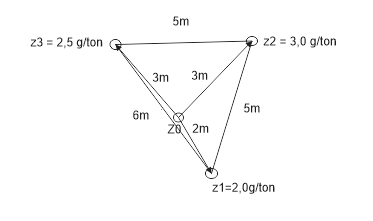
\includegraphics[scale=0.8]{exerc_krig.png}
\end{exercise}